\documentclass[onecolumn, groupedaddress, 10pt]{revtex4-1}
\usepackage[utf8]{inputenc}
\usepackage{amsmath}
\usepackage{amsfonts}
\usepackage{amssymb}
\usepackage{graphicx}											% Use pdf, png, jpg, or eps§ with pdflatex; use eps in DVI
\usepackage[left=2cm, right=2cm, top=2cm, bottom=2cm]{geometry}
\usepackage{dsfont}												% For using C,R,Q,I,N symbols for Rings.
\usepackage{float}												% for controlling the position of objects ie. tables
%\usepackage{breqn}												% For splitting equations using \left and \right across lines
%\usepackage{color}												% For adding color to equations ex.: "/color{red}"
\usepackage[small, bf]{caption}									%Adjust caption size of figures, tables, pictures...
\setlength{\captionmargin}{15pt}
										
\graphicspath{{images/}
              {earthMotionModulationFigure/}
              {images/trial1Results/}}									% folder where images are stored in current directory


% --------------------------- Code for placing two figure side by side ------------------------------------------------------------------
\usepackage{caption}
\usepackage{subcaption}

% --------------------------- Code for the bibliography ---------------------------------------------------------------------------------
\usepackage{natbib}												% For fancy in-text citations
\bibliographystyle{plain}



\begin{document}

\author{Curtis Rau$^{1,2}$}
\author{Colin Gordon$^{1,2}$}
\author{David Witalka$^{1,2}$}
\author{Samuel Akwei-Sekyere$^{1,3}$}
\affiliation{Department of Mathematics$^{1}$ \newline Department of Physics and Astronomy$^{2}$ \newline Neuroscience Program$^{3}$ \newline Michigan State University \newline}

\title{A Novel Method for Removing Cyclic Frequency Modulation in Fourier Space}


\begin{abstract}
By building on the method established in \citep{Deanna}, this paper primarily seeks to introduce the Gustafson algorithm for removing frequency/phase modulation from a signal. The Gustafson algorithm uses the time series data as its input and outputs the original single tone carrier frequency. This method is powerful because it works in the frequency rather than time domain --- which easily allows for filtering of the signal. Here, we will focus on the Gustafson algorithm's applications to LIGO and the search for gravitational waves; nevertheless, there are many other possible applications for the algorithm such as radio wave astronomy and communications systems using frequency modulated signals. Since one of the pertinent issues in any detection algorithm is signal adulteration by noise, we shall also introduce a novel approach to deal with correlated noise from a multichannel perspective.

\end{abstract}

\maketitle

% --------------------------- Code for the Cover Page ---------------------------------------------------------------------------------

\section{Introduction}
General Relativity postulates that information about the spatial distribution of matter in the universe is transmitted via a gravitational field \cite{einstein1990gravitational}. Information regarding changes in mass distribution of the universe propagate through space-time away from the location of that change at the speed of light.  Special events, where the quadrupole moment of the mass distribution changes, emit gravitational radiation \cite{poisson1998gravitational}.  Extremely violent events in the universe can release enough gravitational radiation to be detectable from Earth.

Recently, the Laser Interferometer Gravitational-Wave Observatory (LIGO) obtained the first emperical evidence of gravitational waves. The discovered ripples in space-time by LIGO was a function of the inspiral of two black holes that eventually merged --- an event that consumed approximately three solar masses \citep{abbott}.  It is believed that gravitational wave sources are common in the universe and sources of continuous monochromatic (single frequency) gravitational radiation are predicted to exist --- at least sources with frequencies that persist over many periods \cite{magalhaes1995determination}. Neutron stars have also been implicated as one of the prime sources of gravitational waves.  These stars are expected to emit single frequency waves over long periods of time.  Additionally, it has also been proposed that an appreciable fraction of detectable gravitational wave emitters are binary neutron star systems --- two neutron starts orbiting around each other.

A fundamental challenge to efficient detection of gravitational waves is that orbiting binary neutron star systems invoke frequency modulations which reduce the power of the carrier frequency and distributes it to higher and lower harmonics.  In essence, the power of the signal is dispersed over a range of side-band frequencies; this phenomenon is due to the Doppler effect arising from the Earth's motion relative to the source of the wave. Since the noise observed in the LIGO data is approximately Gaussian and of low signal-to-noise ratio, the extraction of reliable information about gravitational waves is arduous.

In order to calculate the carrier frequency of the wave, consider the wave as one emitted from a source that is megaparsecs away (potentially in other galaxies). By virtue of its distance, the spherical coordinates will not change significantly and the source will move relative to the sun with nearly constant velocity over the time we collect data. By the same token, the Sun will experience the monochromatic wave produced by the source as truly monochromatic, while its detection on the Earth will be in the form of a frequency modulated signal.

\begin{figure*}[ht]
	\centering
	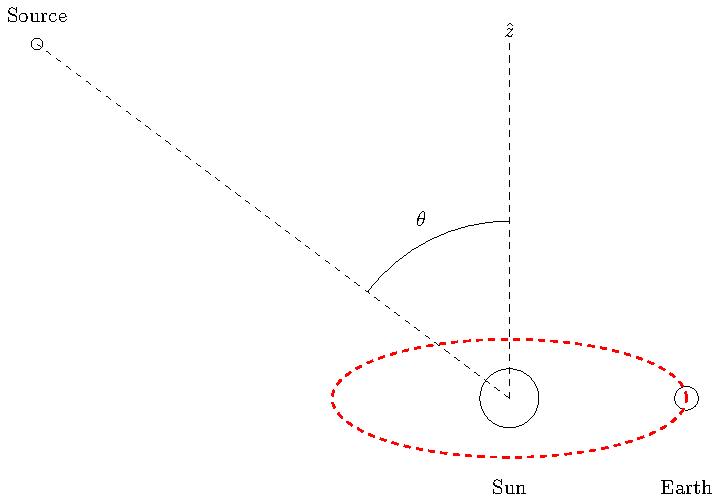
\includegraphics[width=.75\linewidth]{earthMotionModulationFigure.pdf}
	\caption{\label{fig:earthMotionModulationFigure}}
\end{figure*}

By assuming that the wave travels at the speed of light, we can capture it as a Lorentz invariant 4-vector, $\mathbf{K}$ with the carrier frequency being the first entry and the second through fourth entries represent the wave number. In order to transform it in the Earth's frame we apply an instantaneous Lorentz boost on the 4-vector; the instantaneous boost takes the direction of the motion of the Earth and the velocity of the the Earth in orbit into consideration. In our implementation, the Earth's orbit is captured in the $xy$ plane. The 4-vector is written in the perspective that assumes the wave is a plane wave which travels towards the Sun on a trajectory that is on the $xz$ plane: %The matrix with the trigonometric functions projects that 4-vector on a new basis and effectively forcing the second component of the 4-vector to be in the direction of motion of Earth. The matrix with the Betas and gammas is a Lorentz transformation that applies on first and second component. now the 4-vector is in the frame of the Earth. After all of this, we could apply rotations or whatever to change the spatial coordinate system but we only care about the frequency which is invariant under any of those changes.

\begin{align}
\label{eqn: new k}
\mathbf{K} &=
\left( \begin{array}{cccc}
	    \gamma   & -\gamma \beta & 0 & 0 \\
	-\gamma \beta &    \gamma    & 0 & 0 \\
	      0      &       0      & 1 & 0 \\
	      0      &       0      & 0 & 1
\end{array} \right)
\left( \begin{array}{cccc}
	1 &               0             &              0               & 0 \\
	0 & -\sin (\omega_e t + \phi_e) &  \cos (\omega_e t + \phi_e)  & 0 \\
	0 & -\cos (\omega_e t + \phi_e) &  -\sin (\omega_e t + \phi_e) & 0 \\
	0 &               0             &              0               & 1
\end{array} \right)							 
\left( \begin{array}{c}	
	   \omega_0 / c   \\
	- k \sin \theta \\
	        0       \\
	- k \cos \theta    
\end{array} \right)																			\\
&=
\left( \begin{array}{c}
	\gamma \left(\omega_0 / c - \beta k \sin \theta \sin (\omega_e t + \phi_e)\right) \\
	\gamma \left(-\beta \omega_0 / c + k \sin \theta \sin (\omega_e t + \phi_e)\right) \\
	           \gamma k \sin \theta \cos (\omega_e t + \phi_e)           \\
	                           - k \cos \theta
\end{array} \right)   ,
\end{align}

where $\theta$ is the polar angle from the axis perpendicular to the orbit of Earth, $\gamma$ is the Lorentz factor from special relativity, $\omega_e$ is the angular frequency of the Earth's rotation about the Sun, $k$ is the magnitude of the wave number, $c$ is the speed of light and $\beta$ is the velocity of Earth's orbit divided by the speed of light.

From this formulation we can infer that the instantaneous frequency in the Earth's frame can be given by:

\begin{equation}
\omega (t) = \omega_0 \gamma \left( 1 - \beta \sin \theta \sin (\omega_e t + \phi_e) \right). 
\end{equation}

Since the phase refers to the time integral of the frequency, the expression for the wave being sought after is the real part of $h(t)$: 

\begin{align}
h(t)    &= h_0 e^{i \left( \omega' t + \Gamma \cos (\omega_e t + \phi_e) \right)}		\\
\omega' &= \gamma \omega_0															\\
\Gamma  &= \frac{\gamma \beta \omega_0 \sin \theta}{\omega_e}
\end{align}


where $h_0$ is the amplitude of the wave, $\Gamma$ is the modulation index, $\omega_0$ is the frequency of the wave to be detected, $\phi_e$ is the relative phase difference between the Earth's rotation about the Sun and the wave to be detected.


An important note is that $\Gamma$ is a function of only the azimuthal angle of the source with respect to the normal of the gallactic plane. This algorithm will also work perfectly well with any frequency modulated wave produced similar to the above. One likely scenario is that when the compact stars are in a binary system, one or both objects produce waves but the stars rotate around each other causing an analogous phase modulation.  Withal, there could be applications for the Gustafson algorithm in areas outside of gravitational waves in areas such as radio wave astronomy and communications using frequency modulated signals. We attempt to keep the discussion of the algorithm and the results as general as possible for this reason.

\section{The Gustafson Algorithm}
The goal of this paper is to propose a search algorithm that can efficiently detect the presence of frequency modulated waves, while being robust against noise.  A brute force approach to accomplish this is to take the inner product of 

\begin{equation}
h(t) = h_0 e^{i\left( \omega_0 t + \phi_0 + \Gamma \cos (\omega_1 t + \phi_1 ) \right)}
\end{equation}

with the data for different values of $\omega_0$, $\omega_1$, $\phi_0$, $\phi_1$, and $\Gamma$ where $\phi_0$ is the phase of the wave to be detected at $t=0$, with $\omega_1$ and $\phi_1$ being generalizations of $\omega_e$ and $\phi_e$ respectively.  This is effectively a Fourier transform as a function of the four search parameters:

\begin{align}
\hat{f}(\omega_0, \omega_1, \phi_1, \Gamma) = \int f(t) e^{-i\left( \omega_0 t + \phi_0 + \Gamma \cos (\omega_1 t + \phi_1 ) \right)} dt.
\end{align}

It is expected that this approach results in a something like a delta function, or at least a Dirchlet kernel because of discretization, because of the results in the previous section.  The amount of time it will take to perform this computation is $\mathcal{O} (N_tN_{\omega_0}N_{\omega_1}N_{\phi_1}N_\Gamma)$, where $N_t$ denotes the number of data points, and the other $N_x$ is the number of steps in $x$ that the search will take.  Typically for a Discrete Fourier Transform (DFT) the number of steps in frequency is equal to the number of data points: $N_t=N_{\omega_0}=N_{\omega_1}$ \cite{rader1968discrete} \cite[P. 251]{folland}.  Physically, this infers that the frequency resolution of the DFT is proportional to the duration of the time series over which the DFT is taken.  Thus the computation time for the brute force method goes as $\mathcal{O} (N_t^3N_{\phi_1}N_\Gamma)$.  

The case when the signal is buried deep within non-coherent noise is of particular interest.  A conventional method to improve the signal to noise ratio (SNR) is by increasing the number of data points;  this assumes the signal is more periodic than noise. The problem with taking more data however is that computational time of the brute force method is proportional to $N_t^3$.  We will now introduce the Gustafson Algorithm which is roughly a factor of $N_t$ faster than the brute force method.

To derive the Gustafson Algorithm we start by assuming the data $f(t)$ takes on the form of a complex frequency modulated wave. Although the recorded data is real, it will be shown later that starting with the complex wave is perfectly valid.  First, we demodulate the wave and take the Fourier transform of both sides:

\begin{align}
h_0 e^{i\left( \omega_0 t + \phi_0 + \Gamma \cos (\omega_1 t + \phi_1 ) \right)} &= f(t) 												\\
h_0 e^{i\phi_0} e^{i\omega_0 t} &= f(t) e^{-i\Gamma \cos (\omega_1 t + \phi_1)}															\\
h_0 e^{i\phi_0} \mathcal{F}_t \left[ e^{i\omega_0 t} \right] &= \mathcal{F}_t \left[ f(t) e^{-i\Gamma \cos (\omega_1 t + \phi_1)} \right].
\end{align}

Define $\mathcal{F}_t[f(t)](\omega) = \hat{f}(\omega)$. By invoking the convolution theorem yields,

\begin{equation}
\label{eqn:derivation:convolutionThmStep}
\frac{h_0 e^{i\phi_0}}{\sqrt{2\pi}} \delta (\omega_c - \omega) = \hat{f}(\omega) \star \mathcal{F}_t \left[ e^{-i\Gamma \cos (\Omega t + \phi)} \right].
\end{equation}

The Jacobi-Anger Expansion, which comes up often in this paper, has the form \cite{deanna}:

\begin{equation}
\label{eqn:jacobiAnger}
e^{iz\cos (\theta)} = \sum_{n=-\infty}^{\infty} e^{in\pi/2} J_n(z) e^{in\theta}.
\end{equation}

By invoking the previously mentioned expansion, equation \ref{eqn:derivation:convolutionThmStep} becomes

\begin{align}
\label{eqn:derivation:jacobiAngerInsertion}
\frac{h_0 e^{i\phi_0}}{\sqrt{2\pi}} \delta (\omega - \omega_0)
&=
\hat{f}(\omega)
\star \mathcal{F}_t \left[ \sum_{n=-\infty}^{\infty} e^{in\pi/2} J_n(-\Gamma) e^{in(\omega_1 t + \phi_1)} \right].
\end{align}

Even order Bessel Functions are even, and odd order Bessel Functions are odd \cite{kreh}.  Explicitly

\begin{align}
J_n(-z) &= (-1)^n J_n(z)
\end{align}

By employing this fact we observe that

\begin{align}
\mathcal{F}_t \left[ \sum_{n=-\infty}^{\infty} e^{in\pi/2} J_n(-\Gamma) e^{in(\omega_1 t + \phi_1)} \right]
&= \sum_{n=-\infty}^{\infty} (-1)^n e^{in\pi/2} e^{in\phi_1} J_n(\Gamma) \mathcal{F}_t \left[e^{in\omega_1 t} \right]	 \\
&= \frac{1}{\sqrt{2\pi}}\sum_{n=-\infty}^{\infty} e^{in(\phi_1 - \pi/2)} J_n(\Gamma) \delta (\omega - n\omega_1).
\end{align}

In the previous step we used the linearity of the Fourier transform $\mathcal{F}_t[c \cdot f(t)] = c \cdot \mathcal{F}_t[f]$.  Note that \ref{eqn:derivation:jacobiAngerInsertion} becomes

\begin{align}
h_0 e^{i\phi_0} \delta (\omega - \omega_0) = \hat{f}(\omega)
\star
\left[ \sum_{n=-\infty}^{\infty} e^{in(\phi_1 - \pi/2)} J_n(\Gamma) \delta (\omega - n\omega_1) \right].
\end{align}

By performing the convolution,

\begin{align}
\hat{f}(\omega) \star \delta (\omega - n\omega_1) 
&= \int \hat{f}(\omega - \widetilde{\omega}) \delta(\widetilde{\omega} - n\omega_1) d\widetilde{\omega}			\\
&= \hat{f} (\omega - n\omega_1)
\end{align}

brings us to the almost final answer

\begin{align}
h_0 e^{i\phi_0} \delta (\omega - \omega_0) = \sum_{n=-\infty}^{\infty} e^{in(\phi_1-\pi/2)} J_n(\Gamma) \hat{f} (\omega - n\omega_1).
\end{align}

For clarity and later convenience let's have $n\to -n$.  Let us employ a property of the Bessel functions: \cite{kreh}

\begin{align}
\label{eqn:property 2 of Bessel Functions}
J_{-n} (z) &= (-1)^n J_n(z).
\end{align}

This results in the Gustafson Algorithm:

\begin{align}
\label{eqn:gustafsonAlgorithm}
\boxed{h_0 e^{i\phi_0} \delta (\omega - \omega_0) = 2 \sum_{n=-\infty}^{\infty} e^{-in(\phi_1+\pi/2)} J_n(\Gamma) \hat{f} (\omega + n\omega_1)}
\end{align}

An erroneous factor of two has been added to the algorithm which, as we will see, makes it suitable for use with real data.  It is not obvious whether or not this algorithm in its current form can be used on real data because it assumed a complex waveform.  This assumption allowed for a clean demodulation, which is marred if one takes the real of this function.  This is due to the nonlinearity of the real operator as demonstrated by

\begin{align}
\Re \{ a \cdot b \} \neq \Re \{ a \} \cdot \Re \{ b \}; \qquad a,b \in \mathds{C}.
\end{align}

Naively we try plugging the Fourier Transform of the real waveform (eq. \ref{eqn:realFourierTransform}) into the Gustafson Algorithm (eq. \ref{eqn:gustafsonAlgorithm}) and see what happens.  Perhaps unsurprisingly using ether the real or complex waveforms yield the same result.  Notice that the Fourier Transform of the real wave looks very similar to the Fourier Transform of the complex wave (see appendices A and B).  The difference being that the Fourier Transform of the real is symmetric about $\omega=0$ up to a phase factor.  The vectors corresponding to the positive carrier frequency rotate counterclockwise, whereas the vectors corresponding to the negative carrier frequency rotate clockwise (neglecting the rotation due to $\phi_1$ which is the same for both).  \textbf{This phase factor is the reason why the Gustafson Algorithm only picks out the positive value of $\omega_0$.}  If it is unclear what this means refer to figure (\ref{fig:gustafsonAlgoResults}e).  

Now we will try to build an intuitive conceptual model of the Gustafson Algorithm.  The complex numbers form a two dimentional vector field over the real numbers.  This means the Fourier Transform is a collection of three dimentional vectors.  If we plot the vectors in cylindrical coordinates, where the z-axis is frequency, the distance from the z-axis represents the amplitude of that frequency, and the polar angle represents the phase of that frequency component, then we get something like figure (\ref{fig:3dFourierTransform}).

\begin{figure*}[ht]
	\centering
	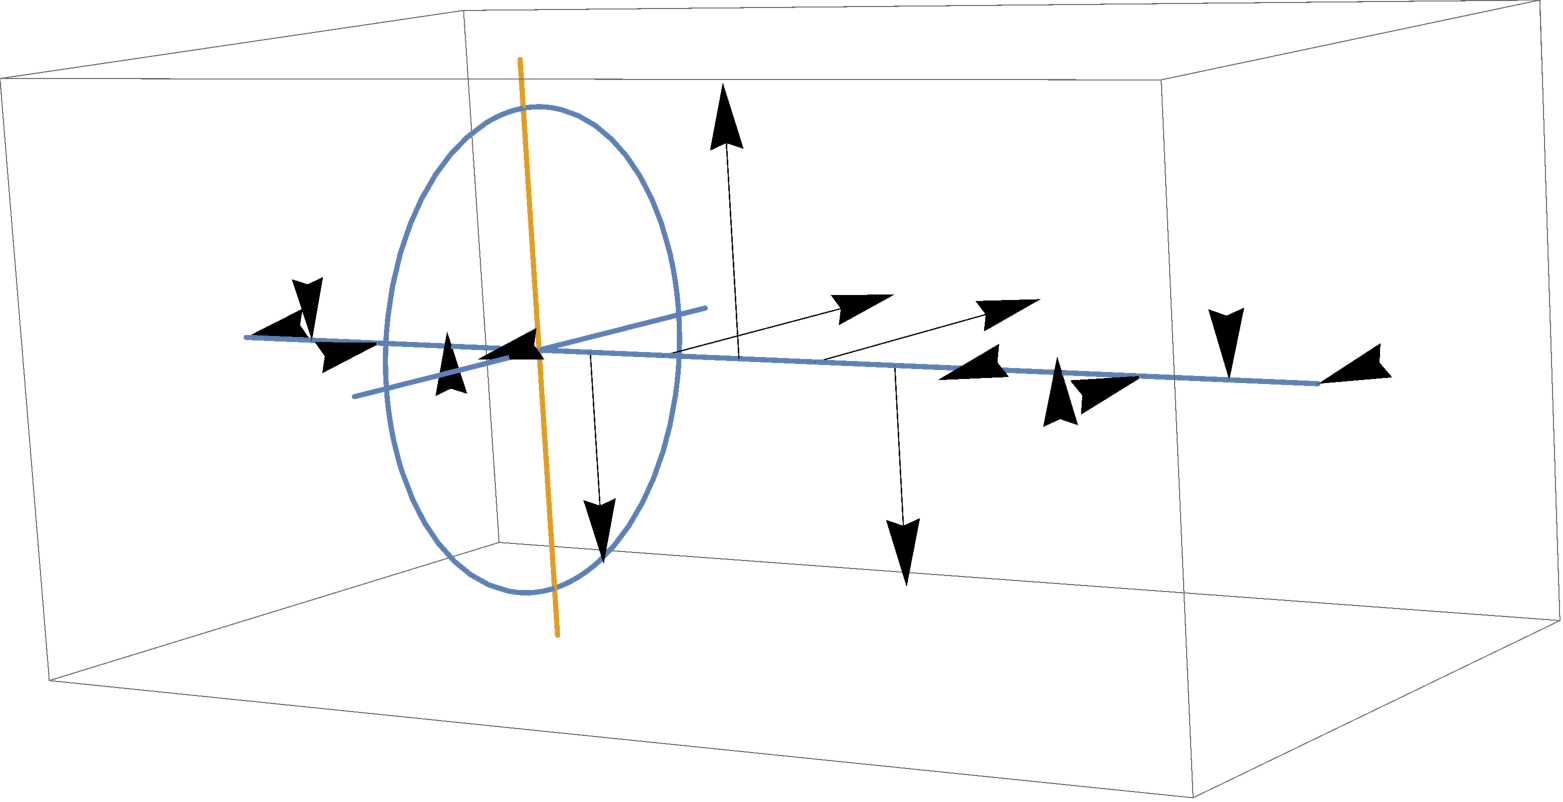
\includegraphics[width=.75\linewidth]{3dFourierTransform.pdf}
	\caption{\label{fig:3dFourierTransform} The 3D representation of the Fourier Transform of the complex waveform.}
\end{figure*}

The Gustafson Algorithm rotates these vectors, multiplies them by a constant, and takes the vector sum of them.  Apparently this vector sum is zero unless the frequency $\omega$ is exactly equal to $\omega_0$ in which case they sum to a vector of infinite length.  The unincluded vectors of the real waveform in figure (\ref{fig:3dFourierTransform}) are symmetric about $\omega=0$ except that they rotate the opposite way around the frequency axis.  This asymmetry in phase is why the Gustafson Algorithm is asymmetric.  It rotates all vectors the same direction.  Apparently the algorithm rotates vectors corresponding to $+\omega_0$ so that they constructively add, whereas it rotates vectors corresponding to $-\omega$ in the wrong direction so they distructively add.


\subsection{The Gustafson Algorithm as a Search Algorithm}
It is not explicitly obvious how The Gustafson Algorithm, Eq. \ref{eqn:gustafsonAlgorithm}, can be used as a search algorithm capable of determining the values $h_0, \omega_0, \omega_1, \phi_0, \phi_1, \Gamma$.  In this section we seek to make obvious what Eq. \ref{eqn:gustafsonAlgorithm} can do. 

Assume the data takes on the real form of a frequency modulated wave.

\begin{align}
\label{eqn:realData}
f(t) = \Re \left\{ h_0 e^{i\left( \omega_0 t + \phi_0 + \Gamma \cos( \omega_1 t + \phi_1 ) \right)} \right\}
\end{align}

Initially we do not know the values of $\omega_0, \omega_1, \phi_0, \phi_1, \Gamma$.  To determine these values we will try the values $\widetilde{\omega}_0, \widetilde{\omega}_1, \widetilde{\phi}_1, \widetilde{\Gamma}$ in the Gustafson Search Algorithm.

\begin{align}
G_{\widetilde{\omega}_0,\widetilde{\omega}_1,\widetilde{\phi}_1,\widetilde{\Gamma}} \left[ \hat{f}(\omega) \right] 
= \sum_{n=-\infty}^{\infty} e^{-in(\widetilde{\phi}_1+\pi/2)} J_n(\widetilde{\Gamma}) \hat{f} (\omega + n\widetilde{\omega}_1)
\end{align}

To see what this will yield we substitute the Fourier Transform of the real of the waveform, equation (\ref{eqn:realFourierTransform}), into the above equation

\begin{align}
G_{\omega_0,\omega_1,\phi_1,\Gamma} \left[ \hat{f}(\omega) \right] = 
&h_0 \sum_{m,n=-\infty}^{\infty} e^{i(m\phi_1-n\widetilde{\phi}_1)} J_n(\widetilde{\Gamma}) J_m (\Gamma)				\nonumber \\
&\times \left[
e^{i(\phi_0 + (m-n)\pi/2)} \delta(\omega - \omega_0 + n\widetilde{\omega}_1 - m\omega_1)
+ e^{-i(\phi_0 + (m+n)\pi/2)} \delta(\omega + \omega_0 + n\widetilde{\omega}_1 - m\omega_1)
\right]
\end{align}

Notice that the erroneous factor of two in front of the Gustafson Algorithm (Eq. \ref{eqn:gustafsonAlgorithm}) has canceled with the factor of one half in front of the Fourier Transform of the real waveform (Eq. \ref{eqn:realFourierTransform}).  This equation is far to complicated to see what is going on, so we will treat it in cases.

%-------------------- w != w0 & w1 != w1~ --------------------

We shall treat this in cases.  

\textbf{Case 1:}  Let us consider the most likely case when $\omega \neq \omega_0$ and $\omega_1 \neq \widetilde{\omega}_1$.  Let us examine the term $\delta(\omega - \omega_0 + n\widetilde{\omega}_1 - m\omega_1)$ in the above equation in detail.  This delta function appears in the double sum and is a function of both $m$ and $n$, so the $n\widetilde{\omega}_1 - m\omega_1$ is changing over the sums whereas the value $\omega - \omega_0$ is constant (not a function of $m$ or $n$).  This delta is non-zero only if

\begin{align}
                0 &= \omega - \omega_0 + n\widetilde{\omega}_1 - m\omega_1		\\
\omega_0 - \omega &= n\widetilde{\omega}_1 - m\omega_1
\end{align}

This can happen twice or never.  By the Euclidean Algorithm, the delta will only be non-zero if

\begin{align}
\gcd \left( \widetilde{\omega}_1, \omega_1 \right) = \omega_0 - \omega
\end{align}

If this is false, then the sum is zero.  If it is true then call the values for $m$ and $n$ that make it true $\pm m_o$ and $\mp n_o$.  So then the sum is 

%Believe I forgot a factor of two out front.
\begin{align}
G_{\widetilde{\omega}_0,\widetilde{\omega}_1,\widetilde{\phi}_1,\widetilde{\Gamma}} \left[ \hat{f}(\omega) \right] = 
h_0 e^{i\phi_0} \delta (0) J_n(\widetilde{\Gamma})J_m(\Gamma) \cos (m\phi_1-n\widetilde{\phi}_1) \times
\left\{
     \begin{array}{lr}
        (-1)^{(m-n)/2} & , m+n $ is even$    \\
		i (-1)^{m-n}   & , m+n $ is odd $
     \end{array}
   \right.
\end{align}

Note that the only way this could give us the true amplitude $h_0 e^{i\phi_0}$ is if $\widetilde{\Gamma} = \Gamma = 0$, $\widetilde{\phi}_1 = \phi_1$, and $m=n=0$.  This is because the Bessel Functions are always less than or equal to one.  The only time equality holds is for $J_0(0)=1$.  Moreover if $m=n=0$ then $\widetilde{\omega}_0 = \omega_0$ which violates our assumption.  Therefore in this case, when $\omega \neq \omega_0$ and $\omega_1 \neq \widetilde{\omega}_1$, the amplitude of the greatest peak will always be less than the true amplitude of the wave.


%-------------------- w = w0 & w1 != w1~ --------------------
\textbf{Case 2:}  Now consider the case when $\omega = \omega_0$ and $\omega_1 \neq \widetilde{\omega}_1$.  The term $\delta(\omega - \omega_0 + n\widetilde{\omega}_1 - m\omega_1)$ will only be non-zero if

\begin{align}
\widetilde{\omega}_1 = \frac{m}{n} \omega_1
\end{align}

This could happen never, or a countably infinite number of times.  If this is false, then the sum is zero.


%-------------------- w != w0 & w1 = w1~ --------------------
\textbf{Case 3:}  Now consider the case when $\omega \neq \omega_0$ and $\omega_1 = \widetilde{\omega}_1$.  The term $\delta(\omega - \omega_0 + n\widetilde{\omega}_1 - m\omega_1)$ will only be non-zero if

\begin{align}
\omega - \omega_0 = (n-m)\widetilde{\omega}_1
\end{align}

This too can happen twice or never.  If this is false then the sum is zero.

%-------------------- w != w0 & w1 = w1~ --------------------
\textbf{Case 4:}  Now consider the case when $\omega = \omega_0$ and $\omega_1 = \widetilde{\omega}_1$.  The term $\delta(\omega - \omega_0 + n\widetilde{\omega}_1 - m\omega_1)$ will only be non-zero if $m=n$ which will happen an infinite number of times.  Thus, the sum becomes

%This treatment does not include the \delta(\omega + \omega_0 + n\widetilde{\omega}_1 - m\omega_1) term of the fourier transform.
\begin{align}
\frac{h_0}{2} e^{i\phi_0} \delta(0) \sum_{n=-\infty}^{\infty} e^{in(\phi_1-\widetilde{\phi}_1)} J_n(\widetilde{\Gamma}) J_n (\Gamma)
\end{align}

\textbf{Case 4a:} Now if we let $\Gamma = \widetilde{\Gamma}$ and $\phi_1 = \widetilde{\phi}_1$ then the sum becomes

\begin{align}
\frac{h_0}{2} e^{i\phi_0} \delta(0) \sum_{n=-\infty}^{\infty} J_n^2 (\Gamma) = \frac{h_0}{2} e^{i\phi_0} \delta(0)
\end{align}

So if we guess every search parameter correctly, $\omega = \omega_0$, $\omega_1 = \widetilde{\omega}_1$, $\Gamma = \widetilde{\Gamma}$, and $\phi_1 = \widetilde{\phi}_1$, then we recover the true amplitude of the wave, as indicated by the Gustafson Algorithm. 


\section{Implementing the Gustafson Algorithm in C++}
\subsection{Calculating Bessel Functions}
Known problems with the algorithm include calculating large order Bessel functions.  The Bessel functions of natural number order are given by

\begin{equation}
J_n(z) = \sum_{m=0}^{\infty} \frac{(-1)^n}{m!(m+n)!} \left( \frac{z}{2} \right)^{2m+n}.
\end{equation}

Hence, calculating the $n$-th Bessel function involves calculating factorials greater than $n!$.  The highest $n$ for which we can store $n!$ in an unsigned long integer type is 20:

\begin{align}
2^{64}-1 = 18,446,744,073,709,551,615 \\
< 21! = 51,090,942,171,709,440,000.
\end{align}

If we are willing to sacrifice some precision to truncation, we can use a double precision floating point integer which allows values upto $1.797,693,134,862,315,7 \cdot 10^{308}$

\begin{align}
170! \approx 7.25 \cdot 10^{306}
< 1.797,693,134,862,315,7 \cdot 10^{308} <
171! \approx 1.24 \cdot 10^{309}
\end{align}

This is not acceptable however, because $\left| J_n(z) \right| \leq 1$.  Therefore, when performing the sum we need precision all the way down to at the very least $0.1$, which would require a mantissa with roughly $308$ digits.  This is not only impractical, but it is by far one of the slowest ways one could calculate values of the Bessel functions.  This whole business of wrestling with factorials can be avoided by calculating the Bessel Functions using Bessel's Equation \ref{eqn:Bessel's Equation} \citep{folland}.

\begin{equation}
\label{eqn:Bessel's Equation}
x^2 J_n''(x) + x J_n'(x) + (x^2 - n^2) J_n(x) = 0
\end{equation}

The standard prescription for numerically solving differential equations is first to discretize the independent variable $x \to x_i = x_{min} + i \cdot \delta x$, and then employ the limit definitions of the derivatives. We will use the three point definitions because their error goes as $\mathcal{O}(\delta x^2)$ rather than using the two point definition with an error that goes as $\mathcal{O}(\delta x)$ \cite{morten}.  Further, because there are only one order of Bessel functions in Bessel's equation, the order is implied by the $n$ that appears, so we will drop the subscript of $n$, $J_n \to J$, and adopt the notation $J(x_i) = J_i$.

\begin{align}
J_i'  &= \frac{J_{i+1} - J_{i-1}}{2 \delta x} \\
J_i'' &= \frac{J_{i-1} - 2J_{i} + J_{i+1}}{\delta x^2}.
\end{align}

Therefore the discretized form of Bessel's equation is

\begin{align}
\label{eqn:Bessel's Equation Discretized}
x_i^2 \frac{J_{i-1} - 2J_{i} + J_{i+1}}{\delta x^2} + x \frac{J_{i+1} - J_{i-1}}{2 \delta x} + (x^2 - n^2) J_i = 0
\end{align}

\begin{align}
\left(\frac{x_i^2}{\delta x^2} - \frac{x_i}{2\delta x}\right) J_{i-1}
	+ \left( \left(1-\frac{2}{\delta x^2}\right)x_i^2 - n^2 \right) J_i
	+ \left(\frac{x_i^2}{\delta x^2} + \frac{x_i}{2\delta x}\right) J_{i+1}
	= 0
\end{align}
where we have collected like terms of $J_i$.

For convenience we define coefficients to simplify the above equation.

\begin{align}
a_i &= \frac{x_i^2}{\delta x^2} - \frac{x_i}{2\delta x} 	\\
b_i &= \left(1-\frac{2}{\delta x^2}\right)x_i^2 - n^2  	\\
c_i &= \frac{x_i^2}{\delta x^2} + \frac{x_i}{2\delta x}
\end{align}

These coefficients can be simplified by using the definition for $x_i$, and taking $x_{min} = 0$.

\begin{align}
a_i &= i   \left( i - \frac{1}{2} \right)				\\
b_i &= i^2 \left( \delta x^2 - 2  \right) - n^2 		 	\\
c_i &= i   \left( i + \frac{1}{2} \right)
\end{align}

In effect, the discretized Bessel's equation with simplified coefficients is

\begin{align}
a_i J_{i-1} + b_i J_i + c_i J_{i+1} = 0
\end{align}

By writing out the system of equations explicitly, we have:

\begin{align}
b_1 J_1 + c_1 J_2                                 &= - a_1 J_0		\\
a_2 J_1 + b_2 J_2 + c_2 J_3                       &= 0				\\
a_3 J_2 + b_3 J_3 + c_3 J_4                       &= 0				\\
                                                  &\vdots				\\
a_{n-1} J_{n-2} + b_{n-1} J_{n-1} + c_{n-1} J_{n} &=   0				\\
a_n J_{n-1} + b_n J_n                             &= - c_n J_{n+1}
\end{align}

This suggests Bessel's equation can be written as a matrix equation:

\begin{align}
\left( \begin{array}{ccccc}
	b_1 & c_1 &         &         &         \\
	a_2 & b_2 &   c_2   &         &         \\
	    & a_3 &   b_3   &   c_3   &         \\
	    &     & \vdots  & \vdots  &         \\
	    &     & a_{n-1} & b_{n-1} & c_{n-1} \\
	    &     &         &   a_n   &   b_n
\end{array} \right)
\left( \begin{array}{c}
	  J_1   \\
	  J_2   \\
	  J_3   \\
	\vdots  \\
	J_{n-1} \\
	  J_n
\end{array} \right)
=
\left( \begin{array}{c}
	  - a_1 J_0   \\
	      0       \\
	      0       \\
	   \vdots     \\
	      0       \\
	- c_n J_{n+1}
\end{array} \right).
\end{align}

This is a tridiagonal matrix system that characterizes a one dimensional differential equation.  It can be easily solved using the standard Thomas Algorithm.  To program this in C++ we need all the arrays to be indexed from 0.  By virtue of this indexing system, we yield:

\begin{align}
\label{eqn:finalDiscretizedBesselMatrixEqn}
\left( \begin{array}{ccccc}
	B_0 & C_0 &         &         &         \\
	A_1 & B_1 &   C_1   &         &         \\
	    & A_2 &   B_2   &   C_2   &         \\
	    &     & \vdots  & \vdots  &         \\
	    &     & A_{N-4} & B_{N-4} & C_{N-4} \\
	    &     &         & A_{N-3} & B_{N-3}
\end{array} \right)
\left( \begin{array}{c}
	  J_1   \\
	  J_2   \\
	  J_3   \\
	\vdots  \\
	J_{N-3} \\
	J_{N-2}
\end{array} \right)
=
\left( \begin{array}{c}
	    - A_0 J_0     \\
	        0         \\
	        0         \\
	     \vdots       \\
	        0         \\
	- C_{N-3} J_{N-1}
\end{array} \right)
\end{align}

\begin{align}
A_i = a_{i+1} &= (i+1)   \left( i + \frac{1}{2} \right)				\\
B_i = b_{i+1} &= (i+1)^2 \left( \delta x^2 - 2  \right) - n^2			\\
C_i = c_{i+1} &= (i+1)   \left( i + \frac{3}{2} \right)
\end{align}

\subsubsection{The Thomas Algorithm}
The Thomas Algorithm is a lightning fast way to solve tridiagonal systems like equation \ref{eqn:finalDiscretizedBesselMatrixEqn}.  The algorithm consists of two steps.  First there is a forward substitution which eliminates the $A_i$'s, and modifies the $B_i$'s and the vector on the right which we will call the source vector $S_i; \quad \forall i \in [0, N-3]$.

\begin{align}
R_i &=   R_i - \frac{A_i}{B_{i-1}} R_{i-1}; 	\qquad \forall i \in [1, N-3]		\\
B_i &\to B_i - \frac{A_i}{B_{i-1}} C_{i-1}; 	\qquad \forall i \in [1, N-3]		\\
S_i &\to S_i - \frac{A_i}{B_{i-1}} S_{i-1}; 	\qquad \forall i \in [1, N-3]
\end{align}

Then there is a backwards substitution eliminating the $C_i$'s, again modifying the $S_i$'s.  Finally we solve for $J_i$.

\begin{align}
R_i &=   R_i - \frac{C_i}{B_{i+1}} R_{i+1}; \qquad \forall i \in [N-4, 0]	\\
S_i &\to S_i - \frac{C_i}{B_{i+1}} S_{i+1}; \qquad \forall i \in [N-4, 0]	\\
J_i &=   \frac{S_{i-1}}{B_{i-1}};           \qquad \forall i \in [N-2, 1]
\end{align}

The time it takes to perform the Thomas Algorithm goes as $N$ \cite{}.



\subsubsection{Boundary Conditions \label{sec:boundaryConditions}}

To solve this second-order differential equation we will need two boundary conditions.  The boundary condition at $x=0$ is simple:

\begin{displaymath}
   J_n(0) = \left\{
     \begin{array}{lr}
       1 & : n = 0     \\
       0 & : n \neq 0
     \end{array}
   \right.
\end{displaymath}

For the other boundary condition we \textit{could} use the asymptotic form of the Bessel functions.  Theorem 5.1 in \cite{folland} states:

\textit{For each $n \in N$ there is a constant $C_n \in R$ such that, if $x \geq 1$, then}

\begin{equation}
\label{eqn:asymtoticBessel}
\left| J_n(x) - \sqrt{\frac{2}{\pi x}} \cos \left( x - \frac{\pi}{4} (2n+1) \right) \right| \leq \frac{C_n}{x^{3/2}}.
\end{equation}

This is an asymptotic expansion, so it is only valid for large values of $x$.  It turns out the accuracy of the solution to Bessel's Equation relies heavily on the accuracy of the endpoint at $x \neq 0$.  Figures \ref{fig:BesselBadBoundary} and \ref{fig:BesselGoodBoundary} illustrate this point quite well.  The conclusion is that the asymptotic form of the Bessel functions is not accurate enough for even fairly large values of $z$.  We can also do

\begin{align}
J_n (z) = \frac{1}{\pi} \int_{0}^{\pi} \cos \left[ z \sin \theta - n \theta \right] d \theta.
\end{align}

Which is computed using a Riemann sum:

\begin{align}
\label{eqn:numericalIntegralBessel}
J_n (z) &\approx \frac{1}{N} \sum_{i=0}^{N+1} \cos \left[ z \sin(i \cdot dx) - n \cdot i \cdot dx \right];
\qquad dx = \frac{\pi}{N}
\end{align}

The function being integrated becomes more oscillatory as $n$ increases.  Numerical analysis shows that $n$ gives the number of zeros the function has  on the interval $(0,\pi)$ for $z=0$.  For $n=0$ the number of zeros is given by $\lfloor \frac{2z}{\pi} \rfloor$.  We want a way to ensure the calculation is accurate regardless of how oscillatory it is, but we also want it to be as fast as possible. So, we use these facts regarding the zeros to ensure there are roughly the same number of integration points between zeros.  By taking the number of (evenly spaced) integration points to be

\begin{align}
\label{eqn:dynamicIntegrationPoints}
N = 100 \cdot (n + 1) \cdot \Bigg \lfloor \frac{2z}{\pi} + 1  \Bigg \rfloor,
\end{align}

we achieved excellent results (accurate consistently to 16 decimal places) for a wide range of $z$ and $n$.  The $+1$'s are to ensure accurate results when $z$ or $n$ are zero.  The algorithm can have problems when $J$ is extremely small.  Then the function can be off by many orders of magnitude, but because it is essentially zero, it does not seem to effect our results when used as a boundary condition for solving Bessel's Differential Equation.

\begin{figure*}[t]
	\centering
	\begin{subfigure}{.5\textwidth}
  		\centering
  		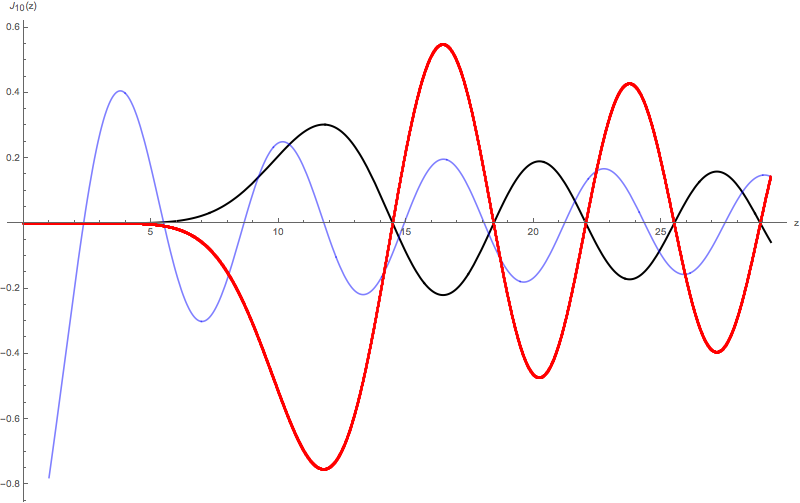
\includegraphics[width=.9\linewidth]{BesselBadBoundary.png}
  		\caption{\label{fig:BesselBadBoundary} Notice how the asymtotic form and the one calculated by our differential equation solver match up at the maximum value for $z$, but do not match up with the true solution.  This has far reaching consequences.  Whatever multiplicative factor the endpoint is off by seems to carry through for every other point.  In this case the multiplicative factor (asymptotic / true) is almost exactly $-2.5$.  Notice how this inverts the solution and makes it $250\%$ larger.}
	\end{subfigure}%
	\begin{subfigure}{.5\textwidth}
  		\centering
  		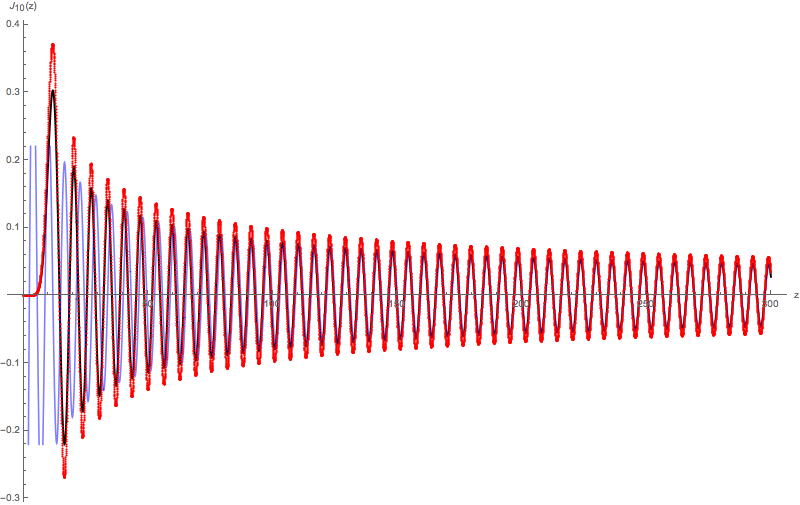
\includegraphics[width=.9\linewidth]{BesselGoodBoundary.png}
  		\caption{\label{fig:BesselGoodBoundary} For much larger values of $z$ the asymptotic form is a better approximation to the true value.  In this case the multiplicative factor (asymptotic / true evaluated at $z=300$) is roughly $1.2$ which results in the solution being roughly $20\%$ larger than it should be.}
	\end{subfigure}
	\caption{The blue curve is the asymptotic form of the bessel functions as given in equation \ref{eqn:asymtoticBessel}, the black curve is $J_{10} (x)$ as given by Mathematica, and the red curve is the one calculated by our differential equation solver.  Note, both of these solutions were calculated using 10,000 points.  Even though the solution in figure \ref{fig:BesselBadBoundary} has 10 times the point density, it is limited in accuracy by the endpoint!}
\end{figure*}

\subsubsection{Calculating Bessel Functions: Results}
The ultimate benchmark for success in calculating Bessel Functions in this manner (using the Thomas Algorithm to solve Bessel's Differential Equation) is to compare it to the standard way of calculating the value at each point using the Riemann Sum (as defined in equation \ref{eqn:numericalIntegralBessel} section \ref{sec:boundaryConditions}).  So how much faster is it?  This depends on the values of $n$ and $z$ because we use a dynamic number of integration points as given by eq. \ref{eqn:dynamicIntegrationPoints}. Table \ref{table:besselSpeed} gives the speed increase for various parameters.

\begin{table}[H]
	\centering
	\begin{tabular}{l || c | c | c }
		                  & Point by Point & Thomas Algo. Solving &  Speed	\\
		Parameters        & Using Integral &  Bessel's Equation   & Increase	\\
		\hline
		\hline
		n = 3             &   0.051786 s   &      0.00013800 s    &   375		\\
		N = 500           &                &                      &			\\
		$z_{max} = 20.0$  &                &                      &			\\
		\hline
		n = 14            &     113.33 s   &       0.003937 s     & 28,785	\\
		N = 50,000        &                &                      &           \\
		$z_{max} = 100.0$ &                &                      &           \\
	\end{tabular}
	\caption{\label{table:besselSpeed} $N$ is the number of points returned, $n$ is the order of the Bessel function, and the points calculated were for $z \in [0,z_{max}]$ }
\end{table}

Figure \ref{fig:selectBesselFunctions} provides three examples of Bessel Functions that were calculated using the Thomas Algorithm to solve Bessel's Equation.

\begin{figure}[H]
	\centering
	\begin{subfigure}{.5\textwidth}
  		\centering
  		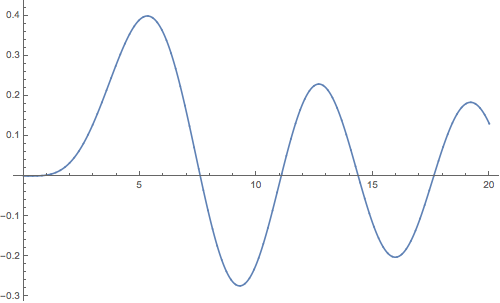
\includegraphics[width=.9\linewidth]{BesselJ4.png}
  		\caption{n=4, numPts=10,000, xMax=20, comptime=0.00082}
	\end{subfigure}%
	\begin{subfigure}{.5\textwidth}
  		\centering
  		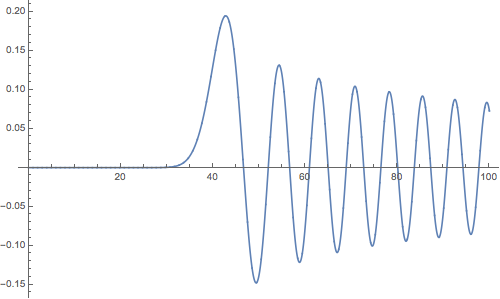
\includegraphics[width=0.9\linewidth]{BesselJ40.png}
  		\caption{n=40, numPts=10,000, xMax=100, comptime=0.00092}
	\end{subfigure}
	\begin{subfigure}{.5\textwidth}
  		\centering
  		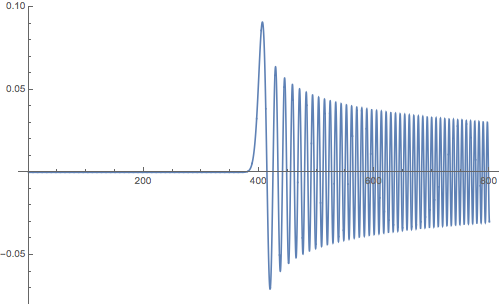
\includegraphics[width=0.9\linewidth]{BesselJ400.png}
  		\caption{n=400, numPts=10,000, xMax=800, comptime=0.00200;  About half the computation time went to calculating the endpoint!}
	\end{subfigure}
	\caption{\label{fig:selectBesselFunctions}}
\end{figure}

In Figure \ref{fig:TA_bessel}, it can be observed that the standard approach and the suggested approach are in agreement except at $n=0,85$.  This is a small subset of the $400,000$ data points generated in $0.33$ seconds (on 5 year old a laptop).  It solved the Bessel differential equation for $4000$ steps in $\Gamma \in (0,100)$, then saved the output, and moved on to solve Bessel's equation for the next value of n until all values of $\Gamma$ and n were solved for.

\begin{figure}[H]
	\centering
	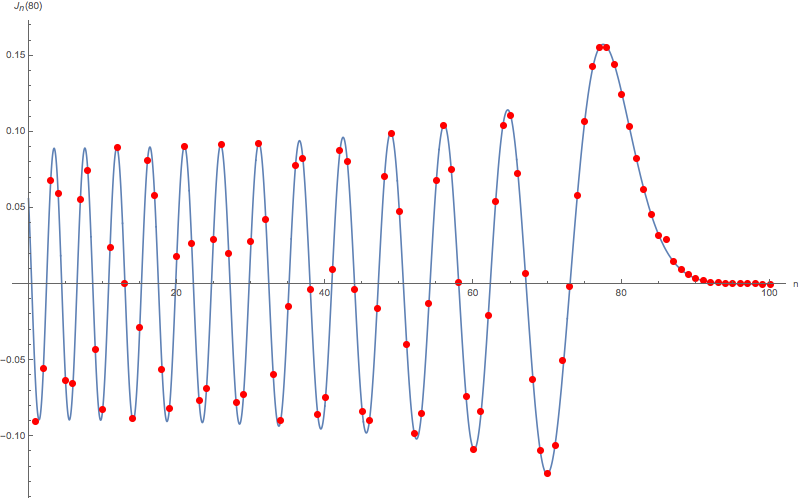
\includegraphics[width=.75\linewidth]{BesselJn80.png}
	\caption{This plot is a plot of $J_n(80)$ for values of $n\in (0,100)$.  The blue curve was generated by the BesselJ function of Mathematica.  The red dots were calculated by our code.  The two sets of data are in excellent agreement at except perhaps $n=0,85$ in which case there is a slight disagreement.  This is a small selection of the $400,000$ data points my code generated in $0.33$ seconds (on 5 year old a laptop).  It solved the Bessel differential equation for $4000$ steps in $\Gamma \in (0,100)$, then saves the output, and moved on to solve Bessel's Equation for the next value of n until all values of $\Gamma$ and n were solved for.\label{fig:TA_bessel} }
\end{figure}

\subsection{Implementing the Gustafson Algorithm}
A practical implementation requires some modifications to the Gustafson Algorithm.  Instead of calculating the negative order Bessel Functions we can use the relation given in equation (\ref{eqn:property 2 of Bessel Functions}).  Restricting the algorithm in this way reduces computation time and memory requirements.

\begin{align}
h_0 e^{i\phi_0} \delta (\omega - \omega_0) 
&= 2 
	\left( 
  		  \sum_{n=-\infty}^{-1} e^{in(-\phi_1+\pi/2)} J_{|n|}(\Gamma) \hat{f} (\omega + n\omega_1)
		+ \sum_{n=0}^{\infty} e^{-in(\phi_1+\pi/2)} J_n(\Gamma) \hat{f} (\omega + n\omega_1)
	\right)																							\\
&= 2 
	\left( 
		J_0(\Gamma) \hat{f} (\omega) + \sum_{n=1}^{\infty} e^{-in\pi/2} J_n(\Gamma) 
		\left[ 
			e^{in\phi_1} \hat{f} (\omega - n\omega_1) + e^{-in\phi_1} \hat{f} (\omega + n\omega_1) 
		\right]
	\right)
\end{align}

-because the FT is symmetric about omega0 it is tempting to simply multiply each sideband by 2 and sum over one side.
-for robustness against noise we want to sum over sidebands on both sides of omega0, not just one.

The infinite limits on the sums must be made finite in any computational implementation.  By the \textit{\textbf{Riemann-Lebesgue Lemma:} If $f\in L^1$, then $\hat{f}(\omega)\to 0$ as $\omega \to \pm \infty$ \citep[P.217]{folland}.} this is well justified.  The question is, what is an appropriate number of sidebands to sum over?  Power is distributed to higher order sidebands as the modulation index increases, thus the number of sidebands to include in the sum should be determined by $\Gamma$.  Upon inspection of the Fourier Transform plotted for various values of $\Gamma$ a trend appears.  Going out from the carrier frequency in ether direction, the power in the sidebands oscillates around, slowly increasing until a maximum is reached, after which the power rapidly goes to zero.  We therefore want to find the value of $n$ that maximizes $J_n(\Gamma)$ for any value of $\Gamma$.  This $n$, multiplied by some constant, gives the number of sidebands to include in the sum.  The following relation, which could not be found in existing literature, was discovered while researching this project.  It will be stated without proof.

\textit{\textbf{Rau's Theorem:} For any $z\in (2,\infty)$ the value of $\nu$ that maximizes $J_\nu (z)$ asymtotically approaches $\nu \to z - \log_\pi (z)$.}

We can use this to calculate how many sidebands we need to sum over.  

\begin{align}
N_{sb} (\Gamma) = 1.5 \, \textsc{round} \left[ \Gamma - \log_\pi ( \Gamma ) \right] + 1
\end{align}

The multiplicative factor of $1.5$ and the additive constant of $1$ are to make the relation work for smaller modulation indicies.  This ensures at least $98\%$ of the power is included in the sum for all values of $\Gamma$.

-the size of the bessel matrix is based on the max value of gamma in the search.
-performing the algorithm suggests that steps in gamma may not need to be very small because we're not stepping over a delta function


\subsubsection{Aliasing and Frequency Folding}
Typically the Discrete Fourier Transform runs over both positive and negative frequencies.  Since the data considered here is real, the negative frequencies contain no additional information and can be ignored.  This restriction cuts the time required to perform the DFT in half.  The frequencies the search has access to are between zero and the Nyquist Frequency.  It is possible for frequencies outside of this range to contain a significant portion of the power.  These frequencies will be folded.  



-only search over positive values of omega0.
-only search over positive values of omega1.


-using aliased sidebands adds some computational overhead in calculating the new frequency.  How much? probably not a lot.




now to calculate the new frequency bin for aliased sidebands. 

for positive frequencies
Calculate the folding zone:

\begin{align}
N_{FZ} = \left\lceil \frac{|f|}{f_{nq}} \right\rceil
\end{align} 

if $N_{FZ}$ is $0$ or $1$, then the frequency is unaliased.  If this is not the case and $N_{FZ}$ is even, then the frequency is aliased and is said to be in an even folding zone.  Frequencies in these zones are mirrored and encure a phase shift of $\pi$.  

\begin{align}
\hat{f}[f] \to -\hat{f}[f_{nq} - f \pmod{f_{nq}} ]
\end{align}

If $N_{FZ}$ is greater than $1$ and odd, then the frequency is aliased and said to be in an odd folding zone.  Frequencies in these zones are translated and do not encure a phase shift.

\begin{align}
\hat{f}[f] \to \hat{f}[f \pmod{f_{nq}} ]
\end{align}




-the number of bins in the fourier transform is (only including positive frequencies)

\begin{align}
N_{FS}=\frac{f_{nq}}{df} + 1
\end{align}


now we need to translate this into c++.  In our fourier transform array 
$f_{nq} \to N_{FS} - 1$
and
$\hat{f}(f_i = df * i) \to \hat{f} (i) $

now we can just change the index:
if n is 0 or 1 do nothing

if n is even: (where i is the ith sideband)
$N_{FS} - 1 - N_{df} * i \pmod{N_{FS} - 1}$

$N_{df} = \lfloor f_1 / df \rfloor $

if n is odd: 
$N_{df} * i \pmod{N_{FS} - 1}$


\section{Results and Discussion}
Since frequency modulated signals may sometimes look like noise in the time domain (see appendix), it is imperative to ascertain that the Gustafson algorithm provides accurate information about the carrier frequency. For this purpose, the Gustafson algorithm was designed to be implemented in Fourier space.

By observing Figures \ref{fig:results_1} and \ref{fig:results2}, we can see that noise added to the frequency modulated signal makes it almost impossible to visually characterize. In practice, most frequency modulated signals encountered --- especially those of astronomical sources and signal susceptible to environmental noise --- are of this form. A simple approach to identifying relevant features of the frequency modulated signal adulterated with noise will be to search for patterns therein. However, since the noise is sampled randomly it is nearly impossible to extract patterns without some form of transformation. The most obvious transform to employ that allows us access the frequencies that compose the noisy signal is its Fourier transform.

In Figures \ref{fig:results3} and \ref{fig:results4} the Fourier transform of the frequency modulated signal and that of the signal adulterated with noise are shown respectively. In the space of the Fourier transform, the frequencies that compose the original signal can be clearly observed. However, this task gets challenging when observing the Fourier transform of the noisy signal. Note that although a high degree of noise has been added, major peaks can still be seen. This is a function of the SNR; with a high enough noise amplitude, the Fourier transform will fail in providing useful information. This suggests that although the Fourier transform is a powerful technique when it comes to ignoring noise within a continuous signal, it is limited by the power of the noise.

\begin{figure}[H]
	\centering
	\begin{subfigure}{.5\textwidth}
  		\centering
  		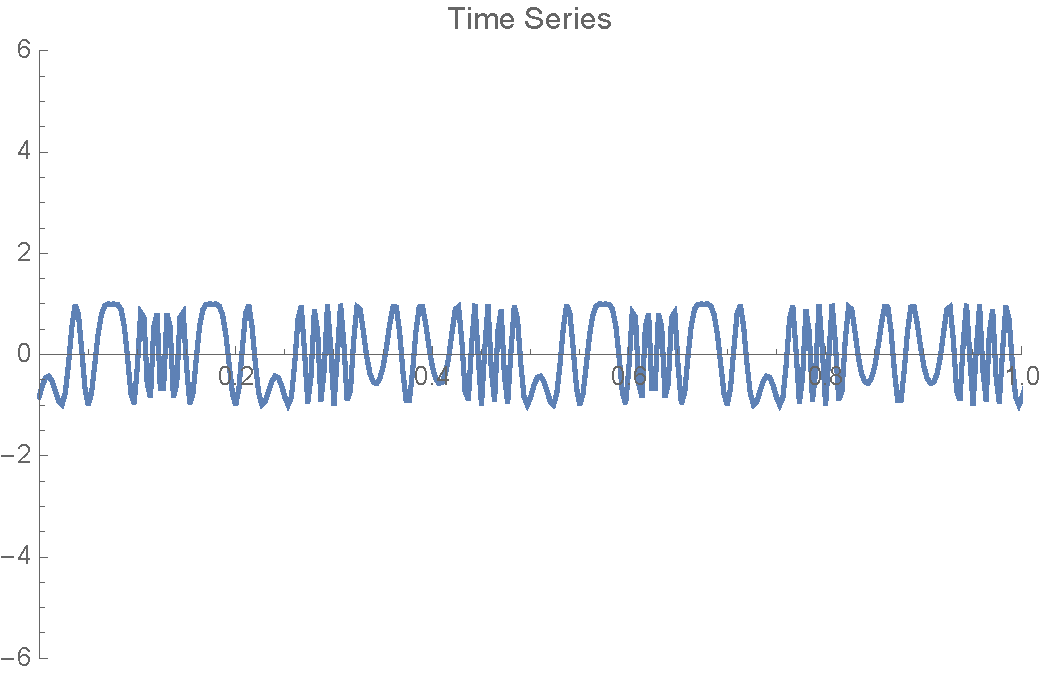
\includegraphics[width=.9\linewidth]{timeSeries.pdf}
  		\caption{\label{fig:results_1}Frequency modulated signal.}
	\end{subfigure}%
	\begin{subfigure}{.5\textwidth}
  		\centering
  		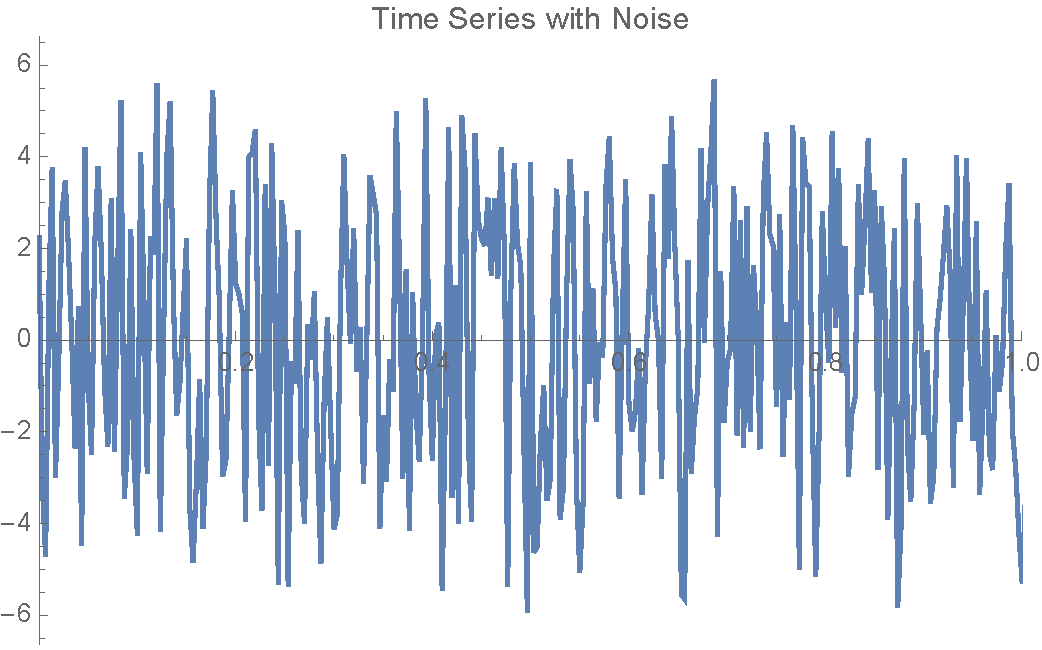
\includegraphics[width=.9\linewidth]{timeSeriesNoise.pdf}
  		\caption{\label{fig:results2}Frequency modulated signal with noise.}
	\end{subfigure}
	\begin{subfigure}{.5\textwidth}
  		\centering
  		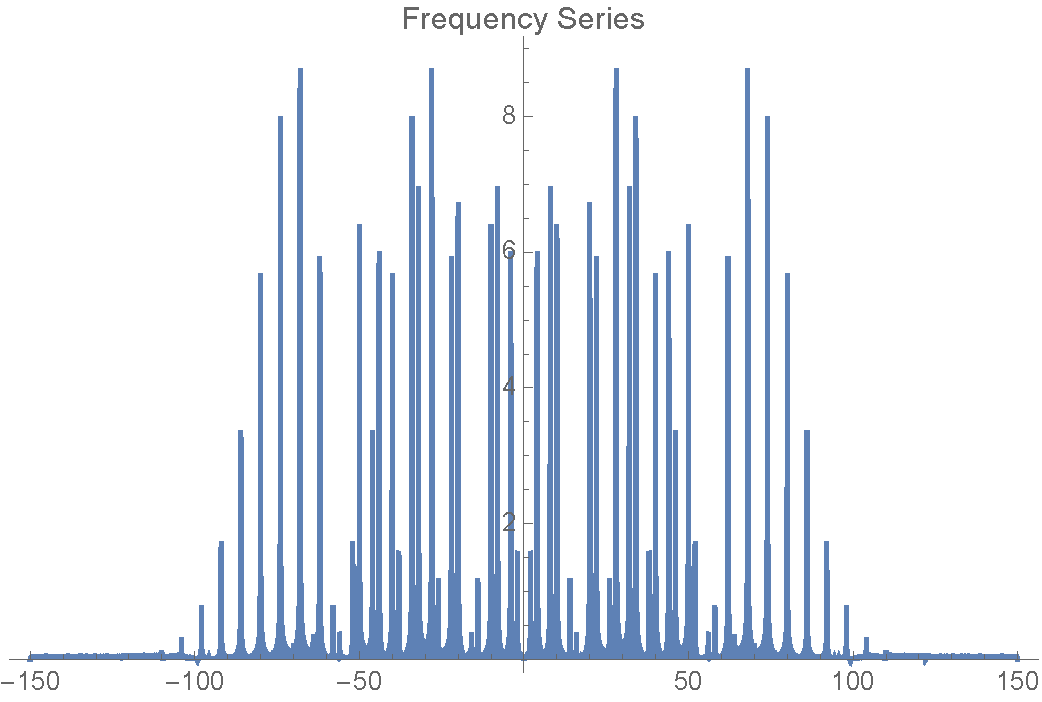
\includegraphics[width=.9\linewidth]{fourierSeries.pdf}
  		\caption{\label{fig:results3} Fourier transform of the frequency modulated signal}
	\end{subfigure}%
	\begin{subfigure}{.5\textwidth}
  		\centering
  		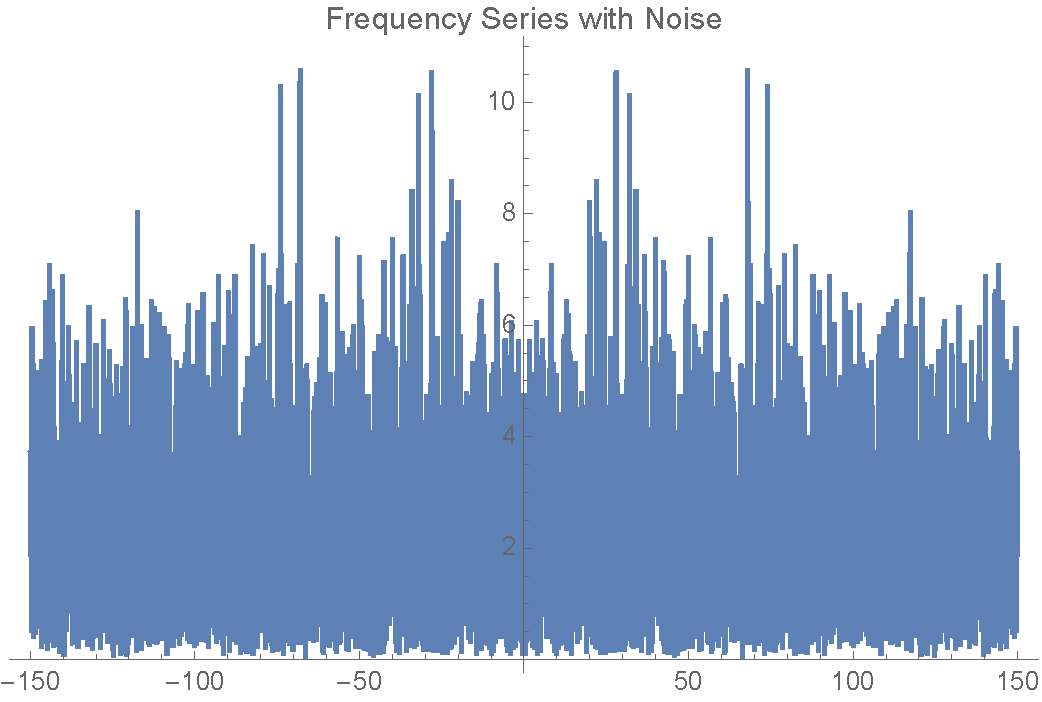
\includegraphics[width=.9\linewidth]{fourierSeriesNoise.pdf}
  		\caption{\label{fig:results4} Fourier transform of (b) above}
	\end{subfigure}
	\caption{\label{fig:} Frequency modulated signal and its noisy version in the time series and Fourier space.  The sampling rate for these traces was 300Hz. The carrier frequency was 20Hz, while the modulaton frequency was 6Hz. It is worth noting that these represent 10 seconds of recording with a modulation index of 10.}
\end{figure}	


To test the  robustness of the Gustafson algorithm against noise, we searched for the carrier frequency, modulation frequency, modulation index and the recipient's angular frequency for they noisy signal provided in Figure \ref{fig:results2}. From Figure \ref{fig:results5} we can see that the Gustafson algorithm appropriately separated out the signal (carrier frequency) from the noise even though it was noise obvious in the corresponding Fourier transform. It is worth noting that the search results in a transform that is asymmetric in frequency; this is a function of the fact that the Gustafson algorithm includes a rotation in Fourier space that is opposite to that of the Fourier transform. With Figure \ref{fig:results6}, it can be observed that the Gustafson algorithm accurately obtained modulation frequency of the noisy signal. Since the search for the carrier frequency and modulation frequency is sensitive, it is important to use small steps; this will aid in preventing one from accidentally skipping over the correct solution. Like the previous results, the Gustafson algorithm was able to extract the correct recipient's angular frequency (Fig. \ref{fig:result7}) and the modulation index (Fig. \ref{fig:result8}) of the frequency modulated signal. Since the search for the modulation index and recipient's angular frequency is relatively smooth, one may take tolerably larger step sizes and still converge to the right solution.

\begin{figure}[H]
	\centering	
	\begin{subfigure}{.5\textwidth}
  		\centering
  		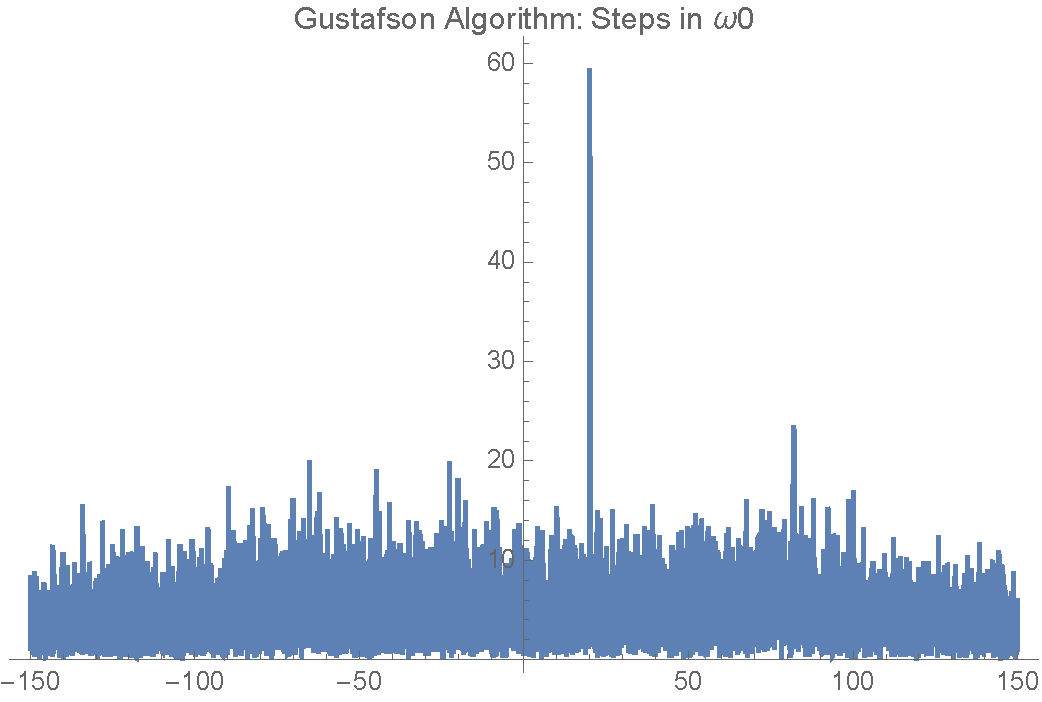
\includegraphics[width=.9\linewidth]{gustafsonAlgoStepInCarrier.pdf}
  		\caption{\label{fig:results5} Extraction of carrier frequency in noisy frequency modulated signal}
	\end{subfigure}%
	\begin{subfigure}{.5\textwidth}
  		\centering
  		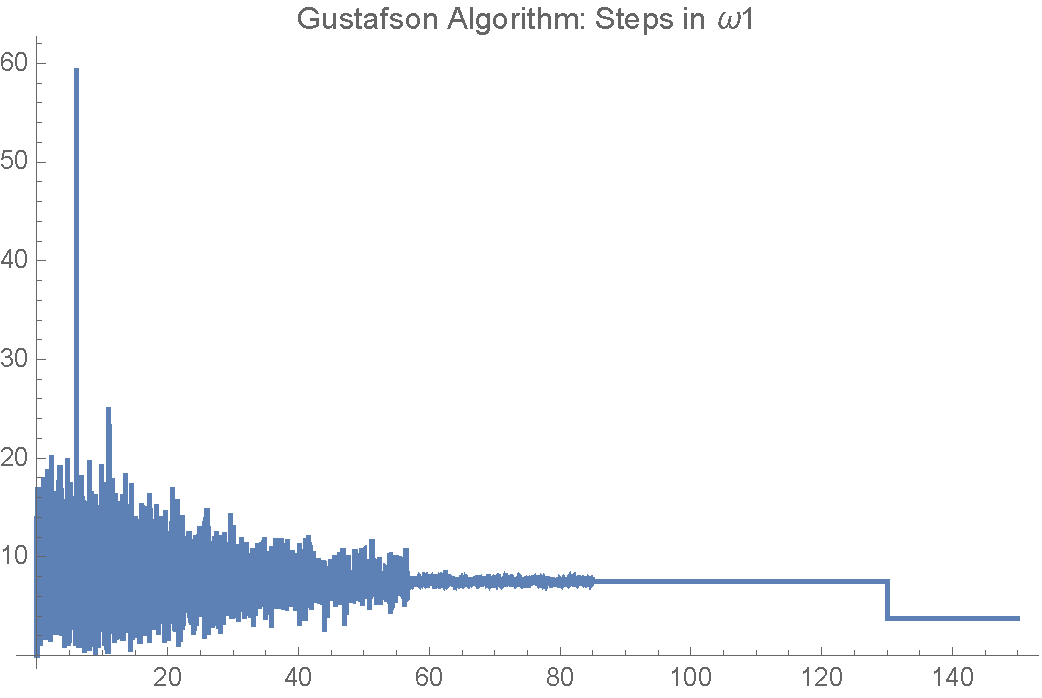
\includegraphics[width=.9\linewidth]{gustafsonAlgoStepInModFreq.pdf}
  		\caption{\label{fig:results6} Detection of the modulation frequency}
	\end{subfigure}
	\begin{subfigure}{.5\textwidth}
  		\centering
  		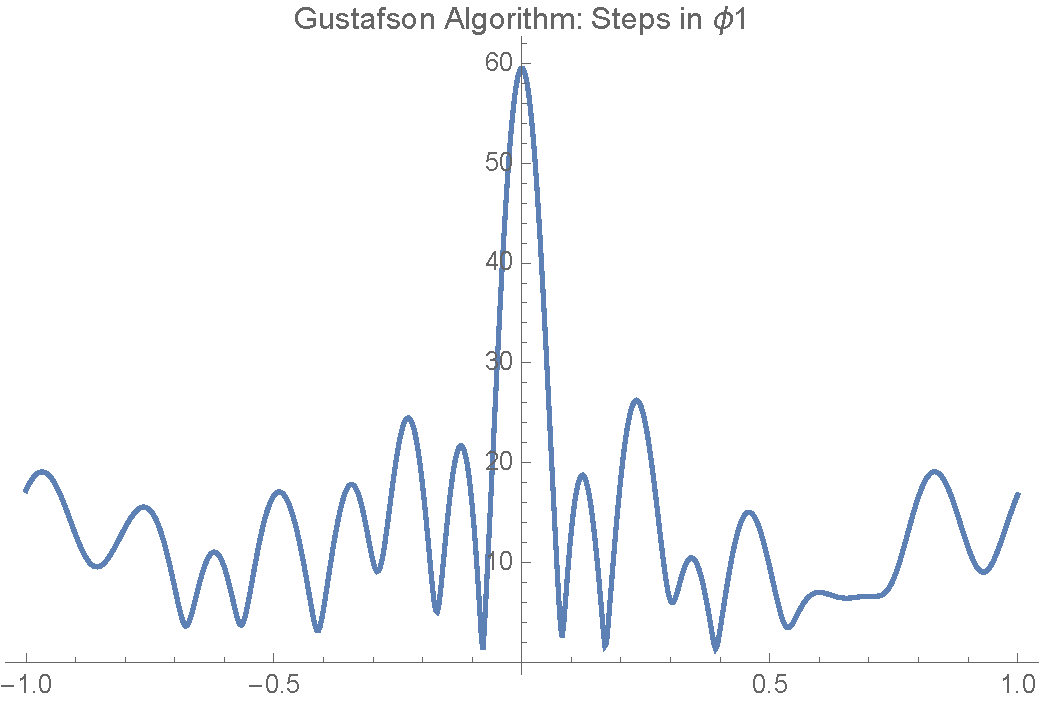
\includegraphics[width=.9\linewidth]{gustafsonAlgoStepInPhi1.pdf}
  		\caption{\label{fig:result7} Search over the recipient's angular frequency}
	\end{subfigure}%
	\begin{subfigure}{.5\textwidth}
  		\centering
  		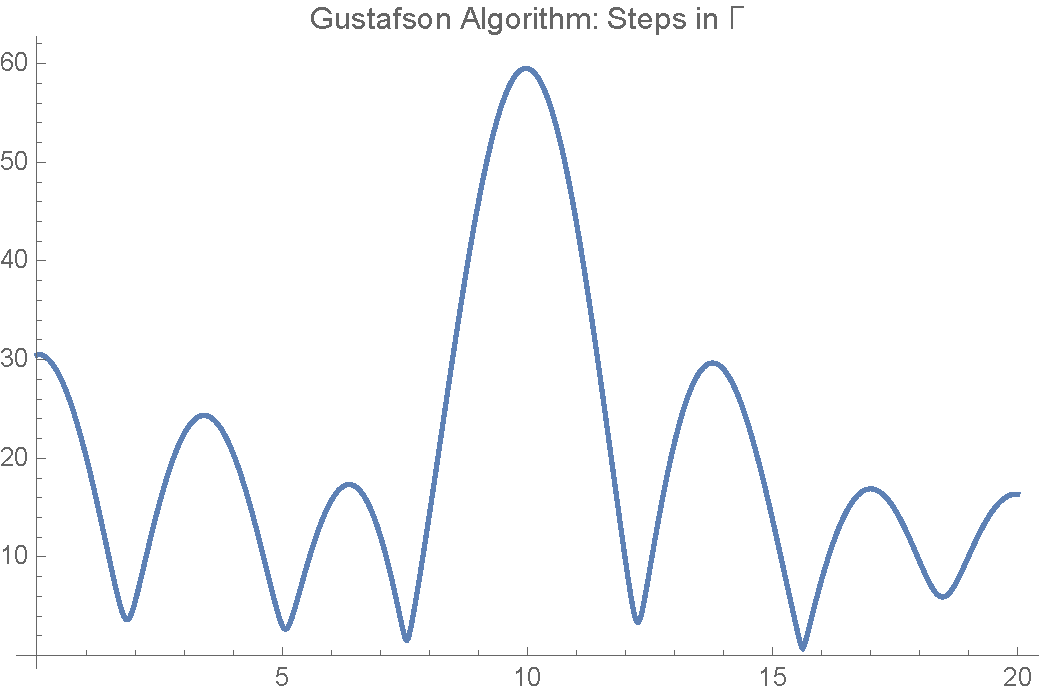
\includegraphics[width=.9\linewidth]{gustafsonAlgoStepInGamma.pdf}
  		\caption{\label{fig:result8} Search over modulation index}
	\end{subfigure}
	\caption{\label{fig:gustafsonAlgoResults} Application of the Gustafson algorithm to the noisy frequency modulated signal illustrated in Fig. \ref{fig:results2}.  Sampling Rate = 300Hz, Carrier = 20Hz, Mod Frequency = 6Hz, Mod Index = 10, Time Series Duration = 10s, SNR = 0.1}
\end{figure}

\section{Conclusion}
In this paper, the Gustafson algorithm has been introduced as well as a novel approach to noise reduction. Although both algorithms presented have been shown to be effective, they may require substantial modifications to be useful in practice. One major draw back of the Gustafson algorithm is the selection of a range of parameters to search over. An investigation of how one can introduce learning procedures such as stochastic gradient descent might be able to provide a steady solution to this issue.


\appendix
\section{The Fourier Transform of The Complex Function}
The results this and the following section are quite surprising.  Looking at the instantaneous frequency of a frequency modulated wave, it takes on every value between $\omega_0 \pm \omega_1$.  There are an uncountable infinite number of frequencies in this band, but essentially every frequency in this band does not appear in the Fourier Transform!  In fact, there are only two or three of these frequencies present in the Fourier Transform.  Moreover the bandwidth for a frequency modulated wave is infinite.  A countably infinite number of frequencies called \textit{sidebands} are evenly spaced at integer multiples of $\omega_1$ from the \textit{carrier frequency} $\omega_0$.  Interestingly for particular values of the \textit{modulation index} $\Gamma$ it is possible for the carrier frequency to not be present in the Fourier Transform!  This occurs at the zeros of the zeroth Bessel Function.

\begin{align}
\mathcal{F}_t \left[ h_0 e^{i\left( \omega_0 t + \phi_0 + \Gamma \cos( \omega_1 t + \phi_1 ) \right)} \right]
&= h_0 e^{i\phi_0} \mathcal{F}_t \left[ e^{i\omega_0 t} e^{i\Gamma \cos(\omega_1 t + \phi_1)} \right]											\\
&= h_0 e^{i\phi_0} \mathcal{F}_t \left[ e^{i\omega_0 t} \right] \star \mathcal{F}_t \left[ e^{i\Gamma \cos(\omega_1 t + \phi_1)} \right]		\\
&= 2 \pi h_0 e^{i\phi_0} \delta(\omega - \omega_0) 
			\star \mathcal{F}_t \left[ \sum_{n=-\infty}^{\infty} e^{in\pi/2} J_n(\Gamma) e^{in(\omega_1 t + \phi_1)} \right]							\\
&= 2 \pi h_0 e^{i\phi_0} \delta(\omega - \omega_0) \star \sum_{n=-\infty}^{\infty} e^{in\pi/2} e^{in\phi_1} J_n(\Gamma) F_t \left[ e^{in\omega_1 t} \right]	\\
&= 2 \pi h_0 e^{i\phi_0} \delta(\omega - \omega_0) \star \sum_{n=-\infty}^{\infty} e^{in(\phi_1 + \pi/2)} J_n(\Gamma) \delta(\omega - n\omega_1)			\\
&= 2 \pi h_0 e^{i\phi_0} \sum_{n=-\infty}^{\infty} e^{in(\phi_1 + \pi/2)} J_n(\Gamma)  \delta(\omega - \omega_0) \star \delta(\omega - n\omega_1)			\\
&= 2 \pi h_0 e^{i\phi_0} \sum_{n=-\infty}^{\infty} e^{in(\phi_1 + \pi/2)} J_n(\Gamma)  \delta(\omega - \omega_0 - n\omega_1)
\end{align}

In this derivation we start by using the linearity of the Fourier Transform, then we invoke the Convolution Theorem, use the Jacobi-Anger Expansion, again use the linearity of the Fourier Transform, and the last few steps are simple Dirac Delta Function manipulations.

\section{The Fourier Transform of The Real-Valued Function}

\begin{align}
\mathcal{F}_t \left[ \Re \left\{ h_0 e^{i\left( \omega_0 t + \phi_0 + \Gamma \cos( \omega_1 t + \phi_1 ) \right)} \right\} \right]
&= \frac{1}{2} \mathcal{F}_t \left[ h_0 e^{i\left( \omega_0 t + \phi_0 + \Gamma \cos( \omega_1 t + \phi_1 ) \right)} 
                        + h_0 e^{-i\left( \omega_0 t + \phi_0 + \Gamma \cos( \omega_1 t + \phi_1 ) \right)} \right]			\\
&= \frac{h_0}{2} \left[ 
  e^{ i\phi_0} \mathcal{F}_t \left[ e^{i\left(  \omega_0 t + \Gamma \cos( \omega_1 t + \phi_1 ) \right)} \right] 
+ e^{-i\phi_0} \mathcal{F}_t \left[ e^{i\left( -\omega_0 t - \Gamma \cos( \omega_1 t + \phi_1 ) \right)} \right] 
\right]
\end{align}

From the previous section we see that

\begin{align}
\mathcal{F}_t \left[ e^{i(\omega_0 t + \Gamma \cos(\omega_1 t + \phi_1))} \right] 
= \sum_{n=-\infty}^{\infty} e^{in(\phi_1 + \pi/2)} J_n(\Gamma)  \delta(\omega - \omega_0 - n\omega_1)
\end{align}

and by replacing $\omega_0$ with $-\omega_0$ and $\Gamma$ with $-\Gamma$, and using the fact that $J_n(-\Gamma) = (-1)^n J_n (\Gamma)$ we also have

\begin{align}
\mathcal{F}_t \left[ e^{i(-\omega_0 t - \Gamma \cos(\omega_1 t + \phi_1))} \right] 
= \sum_{n=-\infty}^{\infty} e^{in(\phi_1 - \pi/2)} J_n(\Gamma)  \delta(\omega + \omega_0 - n\omega_1)
\end{align}

so the Fourier transform of the real part of our frequency/phase modulated signal is

\begin{align}
\begin{split}
\mathcal{F}_t \left[ \Re \left\{ h_0 e^{i\left( \omega_0 t + \phi_0 + \Gamma \cos( \omega_1 t + \phi_1 ) \right)} \right\} \right]
= \frac{1}{2} h_0 \left[ e^{ i\phi_0} \sum_{n=-\infty}^{\infty} e^{in(\phi_1 + \pi/2)} J_n(\Gamma)  \delta(\omega - \omega_0 - n\omega_1) \right.	\\
+ \left. e^{-i\phi_0} \sum_{n=-\infty}^{\infty} e^{in(\phi_1 - \pi/2)} J_n(\Gamma)  \delta(\omega + \omega_0 - n\omega_1) \right]					\\
= \frac{1}{2} h_0 \sum_{n=-\infty}^{\infty} e^{in\phi_1} J_n (\Gamma) \left[ e^{i(\phi_0 + n\pi/2)} \delta(\omega - \omega_0 - n\omega_1) \right.	\\
+ \left. e^{-i(\phi_0 + n\pi/2)} \delta(\omega + \omega_0 - n\omega_1) \right]
\end{split}
\end{align}


%\begin{align}
%\label{eqn:realFourierTransform}
%\Aboxed{\hat{f}(\omega) = 
%\frac{1}{2} h_0 \sum_{n=-\infty}^{\infty} e^{in\phi_1} J_n (\Gamma) \left[ e^{i(\phi_0 + n\pi/2)} \delta(\omega - \omega_0 - n\omega_1)
%+ e^{-i(\phi_0 + n\pi/2)} \delta(\omega + \omega_0 - n\omega_1) \right]}
%\end{align}


\begin{align}
\label{eqn:realFourierTransform}
\hat{f}(\omega) = 
\frac{1}{2} h_0 \sum_{n=-\infty}^{\infty} e^{in\phi_1} J_n (\Gamma) \left[ e^{i(\phi_0 + n\pi/2)} \delta(\omega - \omega_0 - n\omega_1)
+ e^{-i(\phi_0 + n\pi/2)} \delta(\omega + \omega_0 - n\omega_1) \right]
\end{align}

Notice that the Fourier Transform of the real wave looks very similar to the Fourier Transform of the complex wave.  The difference being that the Fourier Transform of the real is symmetric about $\omega=0$ up to a phase factor.  The vectors corresponding to the positive carrier frequency rotate counterclockwise, whereas the vectors corresponding to the negative carrier frequency rotate clockwise (neglecting the rotation due to $\phi_1$ which is the same for both).  \textbf{This phase factor is the reason why the Gustafson Algorithm only picks out the positive value of $\omega_0$.}  If it is unclear what this means refer to figure (\ref{fig:gustafsonAlgoResults}e).

% --------------------------- Code for the bibliography ---------------------------------------------------------------------------------
\bibliography{shgBibliographyCopy}



\end{document}